\subsubsection{Caso d'uso UC8.1 - Consultazione Documentazione API}
\label{UC8.1}
\begin{figure}[ht]
	\centering
	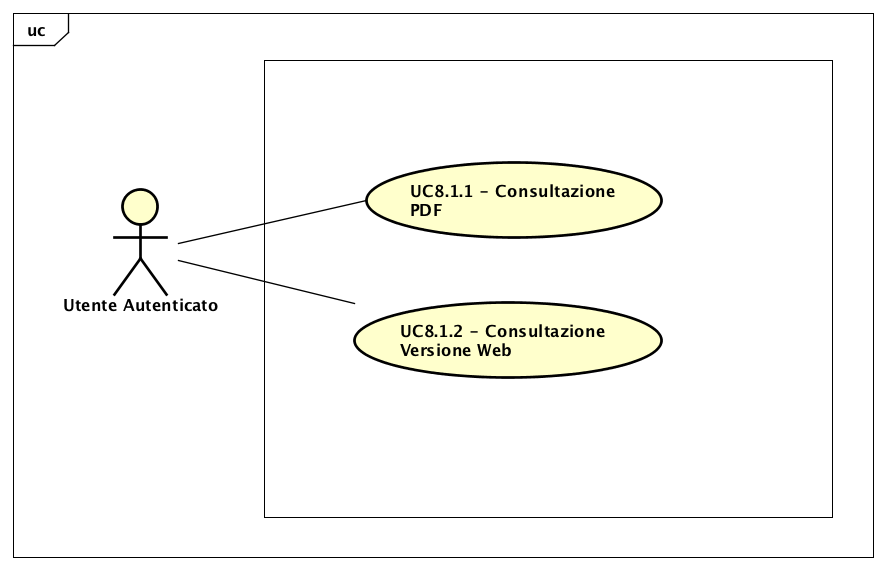
\includegraphics[scale=0.45]{UML/UC8_1.png}
	\caption{UC8.1 - Consultazione Documentazione API}
\end{figure}
\FloatBarrier
\begin{longtable}{ l | p{11cm}}
	\hline
	\rowcolor{Gray}
	\multicolumn{2}{c}{UC8.1 - Consultazione Documentazione API}\\
	\hline
	
	 \textbf{Attori} & Utente autenticato  \\
	\textbf{Descrizione} & L'utente puo' consultare la Documentazione delle API \\
	\textbf{Pre-Condizioni} & L'utente e' autenticato in APIMarket e ha scelto una API dalla lista API\\
	\textbf{Post-Condizioni} & L'utente ha visualizzato la documetazione e ora puo' scegliere un'altra interazione\\
	\textbf{Scenario Principale} & 
	\begin{enumerate*}[label=(\arabic*.),itemjoin={\newline}]
		\item L'utente puo' Consultare la versione PDF della Documentazione (UC8.1.1)
		\item L'utente puo' Consultare la versione Web della Documentazione (UC8.1.2)
	\end{enumerate*}\\
\end{longtable}

